\section{Question 2 -- Motion or Memory?}

\textbf{Implementation summary.} All code is in the repository (notebooks Step 1--6). Moving MNIST is loaded with \texttt{torchvision.datasets.MovingMNIST(split=None)}; videos 0--7999 are used for training, 8000--8999 for validation and 9000--9999 for testing (test videos are numbered 0--999 below). All models were trained and evaluated on Kaggle with an \textbf{NVIDIA Tesla T4} GPU (PyTorch 2.11), with Adam (learning rate $10^{-3}$, no schedule), batch size 32, 30 epochs, final-epoch weights, seeds 0 and 1. Table entries are mean (seed 0, seed 1); errors use three significant figures and scientific notation below $10^{-3}$.

%=====================================================================
\subsection{Setup}

\begin{table}[H]
\centering\footnotesize
\begin{tabular}{@{}llll@{}}
\toprule
& \textbf{Check} & \textbf{Expected} & \textbf{Mine}\\
\midrule
(a) & $\max|M(M(x))-x|$ & 0 & 0 \;(\texttt{torch.equal} = True)\\
(b) & $\max|R^4(x)-x|$ & 0 & 0 \;(\texttt{torch.equal} = True)\\
(c) & $\max|MRM(x)-R^{-1}(x)|$ & 0 & 0 \;(\texttt{torch.equal} = True)\\
(d) & bright pixel of $M(p)$ (frame, row, column) & (7, 10, 43) & (7, 10, 43)\\
(e) & bright pixel of $R(p)$ (frame, row, column) & (7, 43, 10) & (7, 43, 10)\\
(f) & 1$\times$ input / target frames & 1--5 / 6--10 & 1--5 / 6--10\\
(g) & 2$\times$ input / target frames & 1, 3, 5, 7, 9 / 11, 13, 15, 17, 19 & 1, 3, 5, 7, 9 / 11, 13, 15, 17, 19\\
(h) & 3$\times$ input / target frames & 1, 4, 7, 10, 13 / 16, 19 & 1, 4, 7, 10, 13 / 16, 19\\
\bottomrule
\end{tabular}
\caption*{\textbf{Table 1.} Checks of the transformation and window functions (all eight pass).}
\end{table}

\begin{figure}[H]
\centering
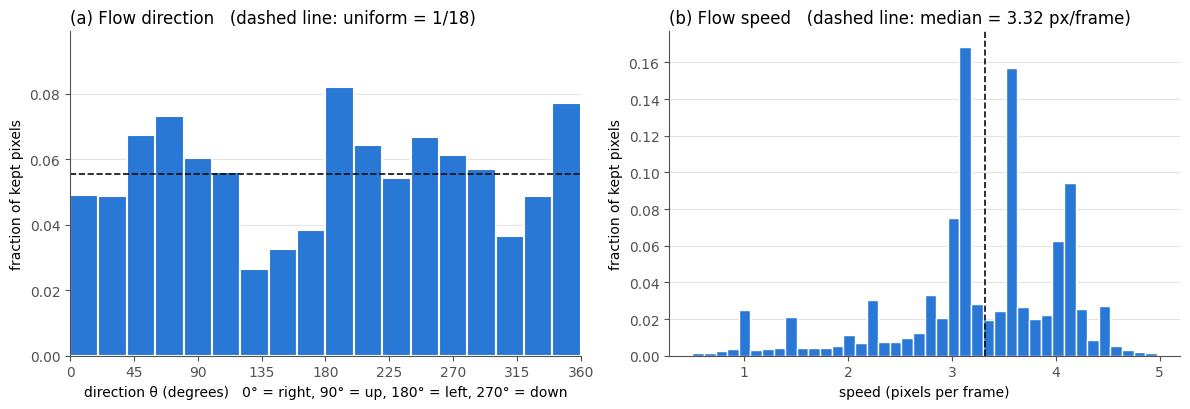
\includegraphics[width=\textwidth]{fig/figure1.png}
\caption*{\textbf{Figure 1.} Farneback optical flow on the first 50 training videos (950 consecutive frame pairs). (a) Flow direction $\theta=\mathrm{atan2}(-d_y,d_x)$, 18 bins of 20$^\circ$, dashed line at 1/18. (b) Flow speed $\sqrt{d_x^2+d_y^2}$ in pixels per frame; dashed line at the median, \textbf{3.32 px/frame}. Both as fractions of the \textbf{103,050 kept pixels}.}
\end{figure}

\qa{Q2.1}
\textbf{Directions.} Yes, as far as the direction of motion is concerned. Figure 1(a) shows that digits in the training data move in every direction: every bin is above zero, the lowest being 0.026 (120--140$^\circ$) and the highest 0.082 (180--200$^\circ$), compared with $1/18\approx0.056$ for a uniform distribution. A mirror changes a direction $\theta$ into $180^\circ-\theta$, and a 90$^\circ$ rotation changes it into $\theta+90^\circ$; for example, a digit moving right (0$^\circ$) moves left (180$^\circ$) after a mirror and upward (90$^\circ$) after a rotation. If every training video were mirrored, the bar at $\theta$ would move to $180^\circ-\theta$; if every video were rotated, every bar would shift by 90$^\circ$. In both cases every bin would still be well above zero, so a mirrored or rotated video contains no direction that is new to a model trained on this data. However, the directions are not equally common, so the transformed histogram would not be identical to the original: for example, after a mirror the 120--140$^\circ$ bin would receive the pixels of the 40--60$^\circ$ bin, and its fraction would rise from 0.026 to 0.067. Some directions would therefore be more common at test time than in training, but none would be unseen. This only concerns motion; mirrored and rotated digits also look different, which is discussed in Q2.2.

\textbf{Speed.} The typical speed is the median, 3.32 px/frame. Playing a video at 2$\times$ means keeping every second frame ($k=2$), so each digit moves twice as far between the frames the model sees: $2\times3.32=6.64$ px/frame. At 3$\times$ ($k=3$) it moves $3\times3.32=9.96$ px/frame. Figure 1(b) contains no kept pixels faster than about 5 px/frame, so these speeds never occur in training: unlike mirrored and rotated motion, faster motion is unfamiliar to a model trained on this data.

\textbf{Overlaps.} No. Optical flow can be wrong where digits overlap, so some pixels get a wrong direction or speed. But overlaps happen only in the few frames where digits cross, so these pixels are a small minority of the 103,050 kept pixels. Their errors spread over many bins: they can change bar heights slightly, but they cannot push a bar to zero or make one much too high, so they act as noise rather than a systematic bias. Even the rarest direction bin holds about 2,700 pixels ($0.026\times103{,}050$), most of them from frames without overlap. The median speed is also robust, because it hardly moves when a small fraction of values is wrong. So the conclusions above do not change.

\qa{Q2.2}
\begin{table}[H]
\centering\small
\begin{tabularx}{\textwidth}{@{}p{2.6cm}YY@{}}
\toprule
\textbf{Transformation} & \textbf{Motion statistics} & \textbf{Digit appearance}\\
\midrule
Mirror & Almost unchanged: each direction $\theta$ becomes $180^\circ-\theta$, but every direction already occurs in training (Q2.1), and the speed is the same. & Changed: digits are reversed left to right (e.g.\ a mirrored 2 or 7). Nearly symmetric digits such as 0, 1 and 8 look almost the same.\\
Rotation by 90$^\circ$ & Almost unchanged: each direction $\theta$ becomes $\theta+90^\circ$. All directions are still familiar, and the speed is the same. & Strongly changed: vertical strokes become horizontal and digits become wider than tall (e.g.\ a 1 becomes a horizontal bar), so almost every digit looks unlike the training digits.\\
Faster (2$\times$, 3$\times$) & Changed: directions stay the same, but the speed rises from 3.32 to 6.64 and 9.96 px/frame, which never occurs in training (Q2.1). & Unchanged: every frame is an ordinary frame of the original video.\\
\bottomrule
\end{tabularx}
\end{table}
Mirror and rotation mainly change the appearance of the digits and keep the motion familiar, whereas faster playback changes only the motion and keeps the appearance familiar. Each transformation therefore changes one factor and holds the other fixed, as in a controlled experiment that changes one variable at a time. Everything else is also held fixed: the same model is tested on the same test videos; mirror and rotation only rearrange pixels (the Table 1 checks give exactly 0); faster playback only skips frames; and the motion rule (straight lines and bounces off the walls) remains valid under all three, so the correct future frames $T(Y)$ are always known and a model that has really learned the motion rule should cope with all three. If a model fails under faster playback, this points to unfamiliar motion, because the digits look normal. If it fails under mirror or rotation, this points to unfamiliar appearance, because the directions and speeds are already familiar. Comparing mirror with rotation adds a further check: both keep the motion familiar, but rotation changes the appearance more, so a larger error under rotation would also point to appearance rather than motion.

%=====================================================================
\subsection{Baseline: ConvLSTM (model A)}

Model A follows the handout: \texttt{pixel\_unshuffle}(4) to a $16\times16$ grid with 16 channels, two ConvLSTM layers (Shi et al., 2015, without peepholes) with 64 hidden channels and $3\times3$ kernels (each layer's four gates come from one convolution on $[u_\tau,h_{\tau-1}]$), a $1\times1$ convolution to 16 channels, \texttt{pixel\_shuffle}(4) and a sigmoid. It is unrolled for 9 steps without teacher forcing (steps 6--9 take its own previous prediction as input); the outputs of steps 5--9 form $\hat Y$. Parameters: 184,576 + 295,168 + 1,040 = \textbf{480,784}. Loss: squared error averaged over pixels and available target frames of each video, then over videos. Training time 11.0 (10.9, 11.2) s per epoch on a T4; final validation $E^{(5)}$ 0.0222 (seed 0) and 0.0218 (seed 1).

\begin{figure}[H]
\centering
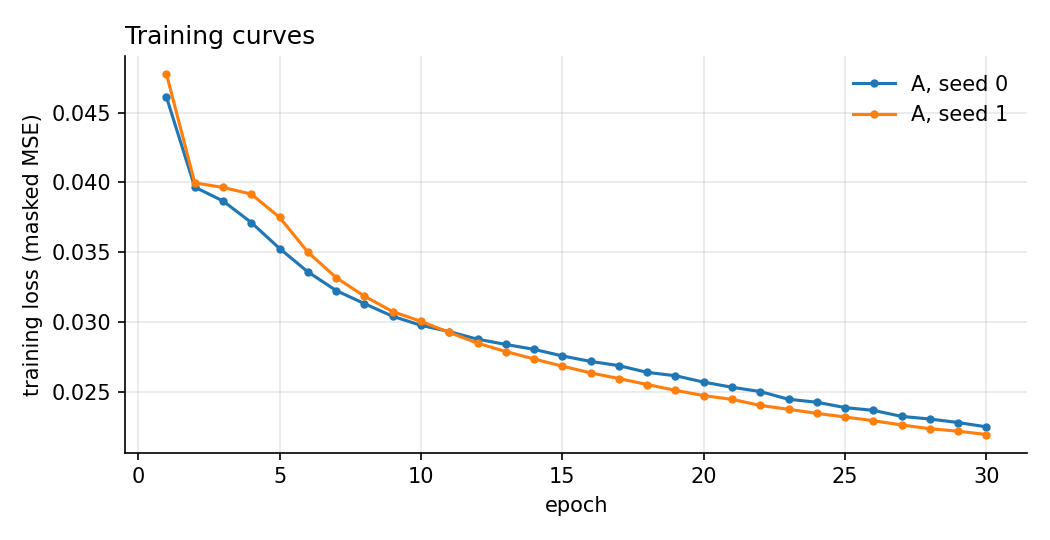
\includegraphics[width=0.62\textwidth]{fig/curves_A.png}
\caption*{\textbf{Figure S1.} Training loss of model A (both seeds). (Supplementary; not a handout figure.)}
\end{figure}

\qa{Q2.3}
Model A's reach is \textbf{8 original pixels per time step} along rows and columns (about 11.3 px diagonally). The reasoning:
\begin{enumerate}
\item \textbf{Patch size.} \texttt{pixel\_unshuffle}(4) folds each $4\times4$ patch into one cell of a $16\times16$ grid, so neighbouring cell centres are 4 original pixels apart: moving one cell means moving 4 px. Following the conventions, the patch width itself is not added, and unshuffle, shuffle and the $1\times1$ output convolution move no information.
\item \textbf{Kernel size.} All four gates of a ConvLSTM layer come from one $3\times3$ convolution on the input and the previous hidden state. A $3\times3$ kernel lets each cell see only itself and its 8 neighbours, so one convolution moves information at most 1 cell. The other gate operations ($\sigma$, $\tanh$, $\times$, $+$) act on each cell separately and move nothing. So each layer moves information at most 1 cell per step.
\item \textbf{Number of layers.} The two layers are stacked: the path from the new input $u_\tau$ passes through the layer-1 convolution and then the layer-2 convolution, so it moves 2 cells.
\item \textbf{Recurrence.} The previous states enter through the same convolutions. The path from $h^{(1)}_{\tau-1}$ passes through both convolutions (2 cells); the path from $h^{(2)}_{\tau-1}$ passes only through the layer-2 convolution (1 cell). The cell states $c$ are updated cell by cell, so they add nothing. The recurrence lets information travel further over several steps, but each single step adds at most 2 cells.
\end{enumerate}
The longest paths (from $u_\tau$ and from $h^{(1)}_{\tau-1}$) move 2 cells $=2\times4=$ \textbf{8 px} along a row or column. Because a $3\times3$ kernel also reaches diagonal neighbours, information can move 2 cells in both directions at once: $\sqrt{8^2+8^2}=8\sqrt2\approx11.3$ px. So in one update, the network can connect a digit's old position (held in its state) with its new position only if the digit moves at most about 8 px horizontally and 8 px vertically per step.

\begin{table}[H]
\centering\small
\begin{tabular}{@{}lcccccccc@{}}
\toprule
\textbf{Model} & \textbf{MSE$_1$} & \textbf{MSE$_2$} & \textbf{MSE$_3$} & \textbf{MSE$_4$} & \textbf{MSE$_5$} & \textbf{$E^{(5)}$} & \textbf{Params} \\
\midrule
A & \makecell{0.0172\\[-1pt]{\tiny(0.0175, 0.0170)}} & \makecell{0.0205\\[-1pt]{\tiny(0.0208, 0.0203)}} & \makecell{0.0228\\[-1pt]{\tiny(0.0231, 0.0225)}} & \makecell{0.0245\\[-1pt]{\tiny(0.0248, 0.0242)}} & \makecell{0.0262\\[-1pt]{\tiny(0.0264, 0.0259)}} & \makecell{0.0222\\[-1pt]{\tiny(0.0225, 0.0220)}} & 480,784 \\
Blank & 0.0426 & 0.0426 & 0.0426 & 0.0425 & 0.0425 & 0.0426 & 0 \\
Copy-last & 0.0492 & 0.0604 & 0.0669 & 0.0708 & 0.0732 & 0.0641 & 0 \\
\bottomrule
\end{tabular}
\caption*{\textbf{Table 2.} Test set, 1$\times$, $t=1$. Model A: mean (seed 0, seed 1).}
\end{table}

\begin{figure}[H]
\centering
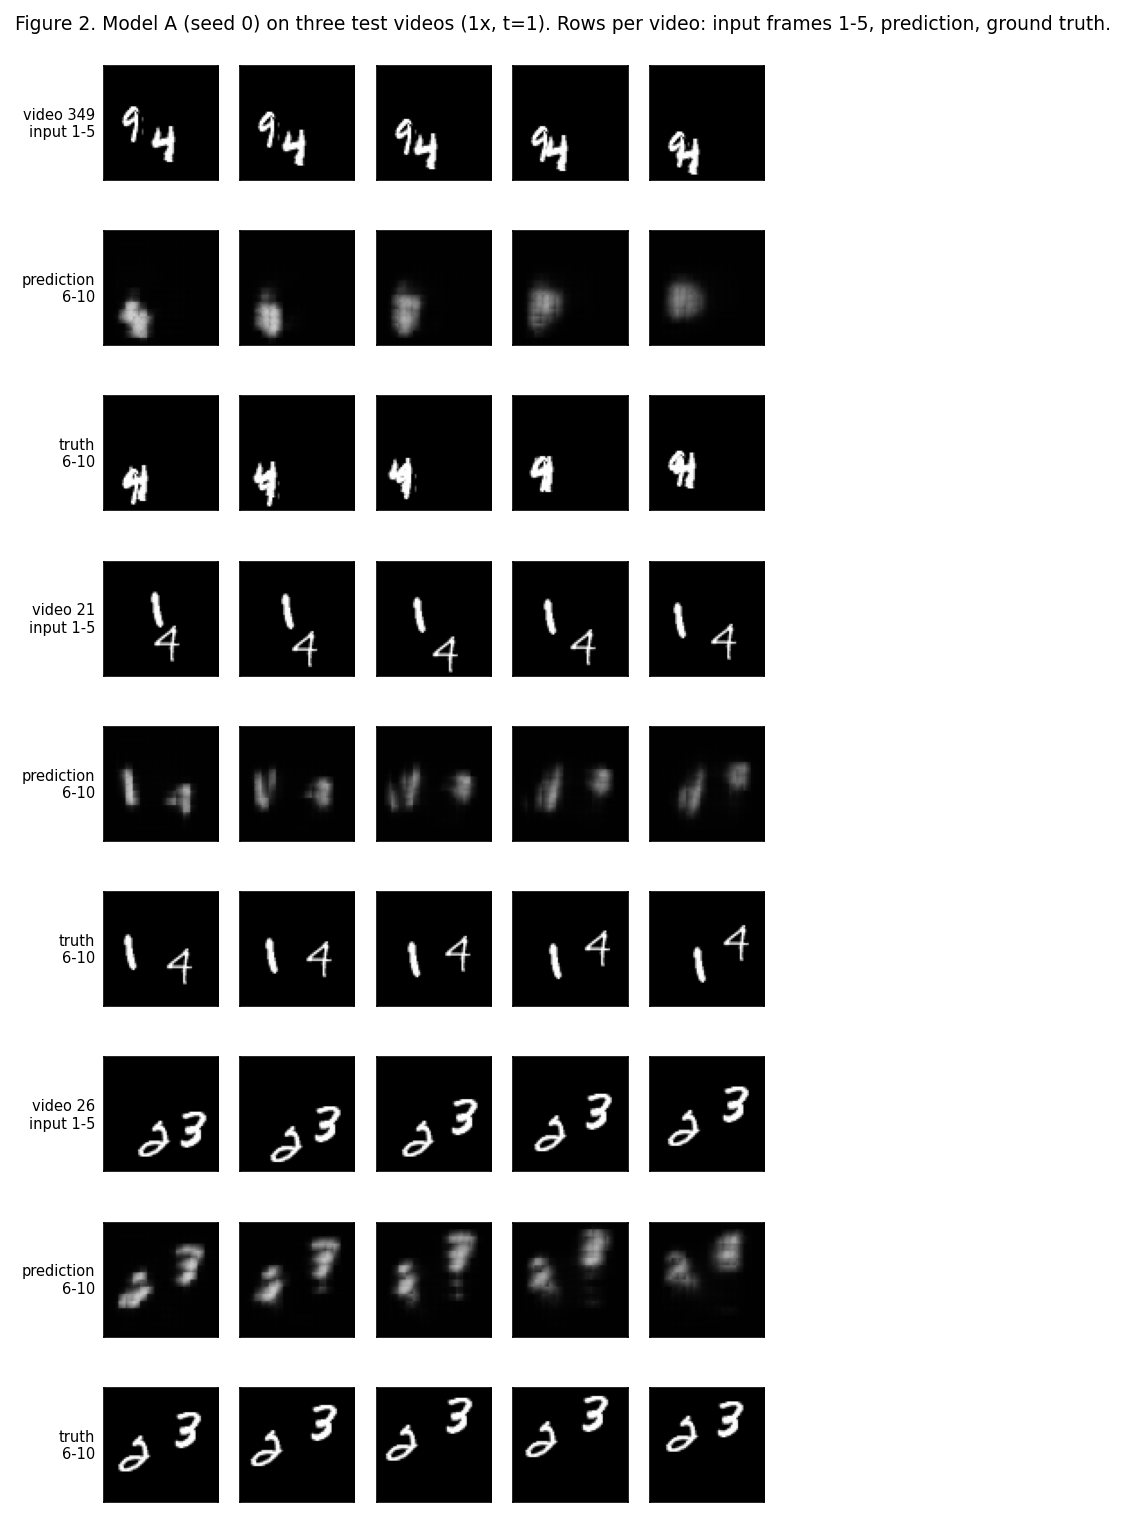
\includegraphics[width=0.62\textwidth]{fig/figure2.png}
\caption*{\textbf{Figure 2.} Model A (seed 0) on test videos 349 (digits overlapping), 21 and 26: input frames 1--5, prediction of frames 6--10, ground truth.}
\end{figure}

\qa{Q2.4}
Model A clearly beats both reference predictors. Its $E^{(5)}$ is 0.0222 (0.0225, 0.0220), about 2$\times$ lower than Blank (0.0426) and about 3$\times$ lower than Copy-last (0.0641), and it is lower than both at every horizon (Table 2). The two seeds differ by only about 2\%, so the result is reliable. Copy-last is worse than Blank even though it looks like a sensible guess, because of the double penalty: the digits move about 3.3 px per frame and their strokes are thin, so a copied digit lands mostly in the wrong place and is wrong twice, dark where the digit really is and bright where it no longer is. Blank is only wrong once, where the digit is.

Model A's error grows steadily with the horizon, from MSE$_1=0.0172$ to MSE$_5=0.0262$ (about +50\%), while Blank stays flat at about 0.0426; even at $h=5$ model A is still well below it. Figure 2 shows why: at $h=1$ the digits are in the right places and still recognisable, but they become blurrier and fainter at every step. From step 6 on the model feeds its own predictions back as input, so small errors build up, and it becomes less certain where each digit will be. Under squared error the best prediction under uncertainty is an average of the possible positions, which is a blur; a blur costs less than committing to one sharp guess that might be wrong, for the same double-penalty reason as Copy-last. In videos 21 and 26 the blobs still roughly follow the true positions, so the motion is tracked even though the digits' shapes are lost.

When digits overlap, the prediction breaks down further. In video 349 the 9 and the 4 overlap in the last input frames, and model A merges them into a single blurry blob: in the prediction one can no longer tell which digit is which, and the model does not follow each digit's own motion.

\qa{Q2.5} \emph{(written before running any experiment in Testing the Baseline; reproduced unedited)}

By ``pass'' I mean that the error on transformed videos, $E_T$, stays close to the normal error $E$.

\textbf{Mirror:} I predict that model A will pass the mirror test. Figure 1(a) shows that every direction already occurs in the training data, so mirrored motion is not new to the model. A mirror also changes the digits only a little: it reverses them left to right, and many strokes still look similar.

\textbf{Rotation:} I predict that model A will also pass the rotation test. Again, every direction already occurs in training (Figure 1(a)), and a rotation does not change the speed. Since rotation, like the mirror, keeps the motion familiar, I expect the same result as for the mirror.

\textbf{Speed:} I predict that model A will work at 1$\times$ and break down at 2$\times$ and higher. At 1$\times$, digits move about 3.32 px per step, the typical training speed (the median in Figure 1(b)). At 2$\times$ and 3$\times$ they move 6.64 and 9.96 px per step, and these speeds are rare in training (Figure 1(b)), so the model has hardly seen motion this fast. My reach estimate (Q2.3) is 8 px per step along rows and columns. At 2$\times$, 6.64 px is still inside this reach, so I expect the breakdown at 2$\times$ to come from the unfamiliar speed rather than from the reach. At 3$\times$, 9.96 px is also beyond the reach (except for nearly diagonal motion, which can reach up to about 11.3 px), so both reasons apply.

%=====================================================================
\subsection{Testing the baseline}

\begin{table}[H]
\centering\small
\begin{tabular}{@{}lccccc@{}}
\toprule
\textbf{Model} & \textbf{$E^{(5)}$} & \textbf{$C_M$} & \textbf{$E_M$} & \textbf{$C_R$} & \textbf{$E_R$} \\
\midrule
A & \makecell{0.0222\\[-1pt]{\tiny(0.0225, 0.0220)}} & \makecell{0.00163\\[-1pt]{\tiny(0.00155, 0.00171)}} & \makecell{0.0228\\[-1pt]{\tiny(0.0231, 0.0226)}} & \makecell{0.00288\\[-1pt]{\tiny(0.00254, 0.00321)}} & \makecell{0.0240\\[-1pt]{\tiny(0.0240, 0.0239)}} \\
Blank & 0.0426 & 0 & 0.0426 & 0 & 0.0426 \\
Copy-last & 0.0641 & 0 & 0.0641 & 0 & 0.0641 \\
\bottomrule
\end{tabular}
\caption*{\textbf{Table 3.} Consistency gaps and transformed errors (test set, 1$\times$, $t=1$). Model A: mean (seed 0, seed 1).}
\end{table}

\begin{figure}[p]
\centering
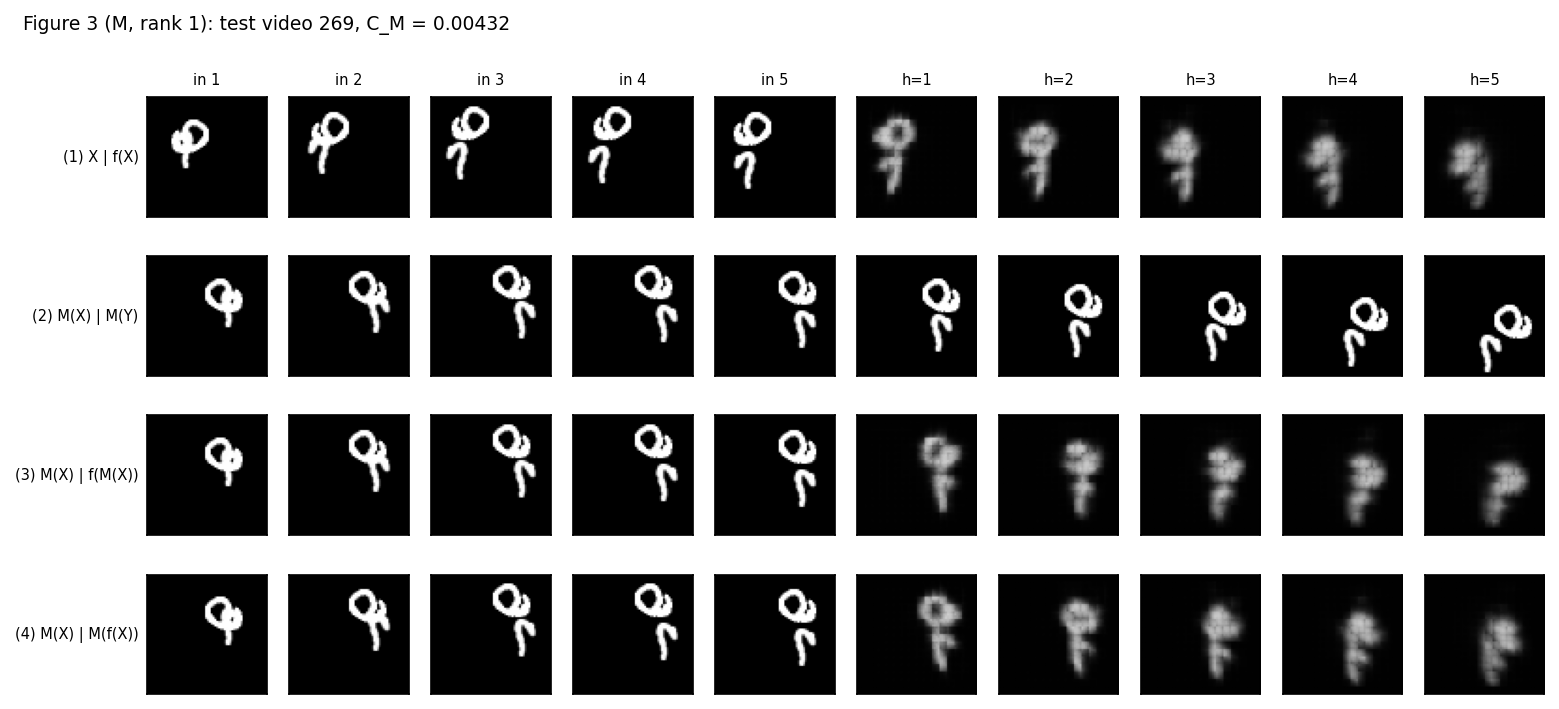
\includegraphics[width=0.93\textwidth]{fig/figure3_M_rank1_video269.png}\\[2pt]
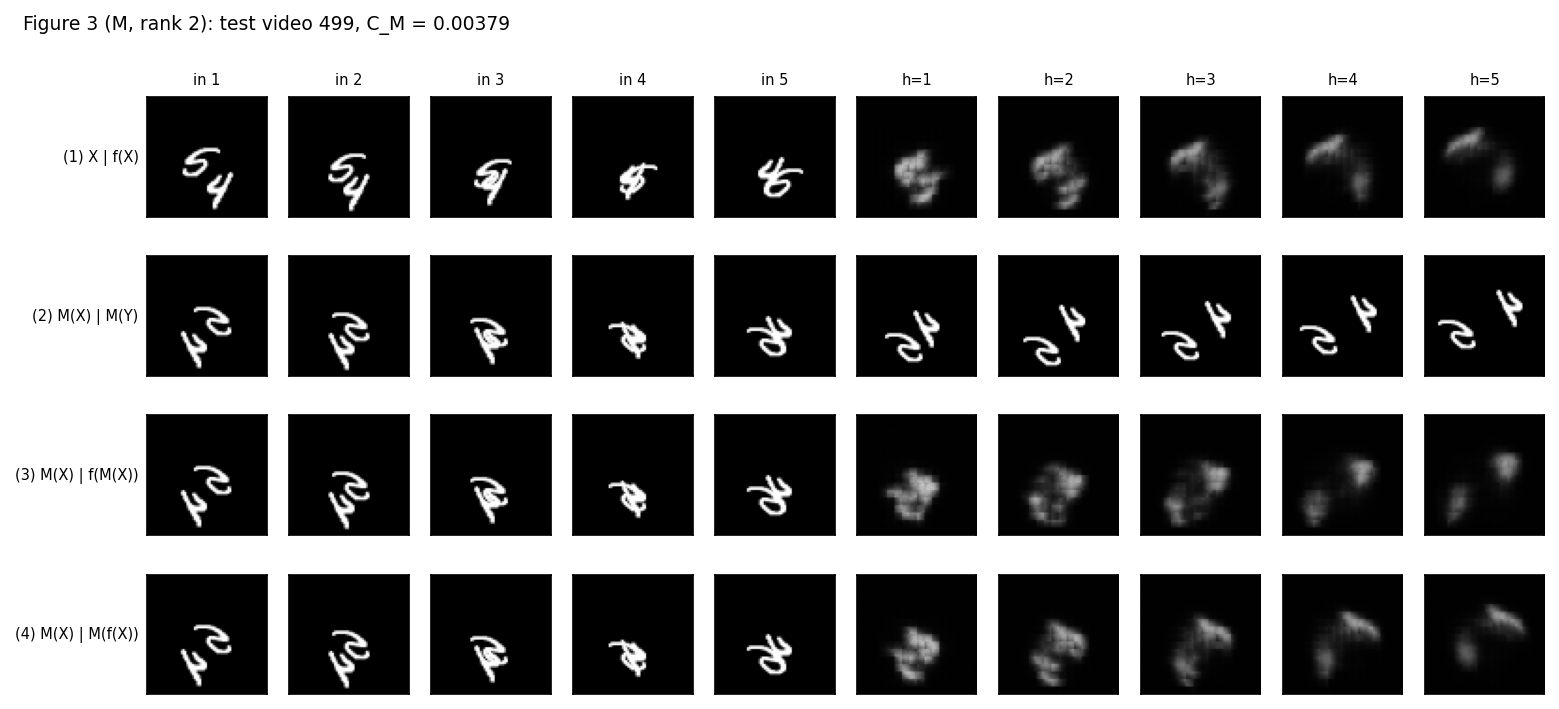
\includegraphics[width=0.93\textwidth]{fig/figure3_M_rank2_video499.png}
\caption*{\textbf{Figure 3 (part 1).} The two test videos with the largest per-video $C_M$ for the seed-0 model A (videos 269 and 499). Rows: (1) $X\mid f(X)$, (2) $M(X)\mid M(Y)$, (3) $M(X)\mid f(M(X))$, (4) $M(X)\mid M(f(X))$. GIFs: \texttt{gifs/figure3\_M\_rank1\_video269.gif}, \texttt{gifs/figure3\_M\_rank2\_video499.gif}.}
\end{figure}
\begin{figure}[p]
\centering
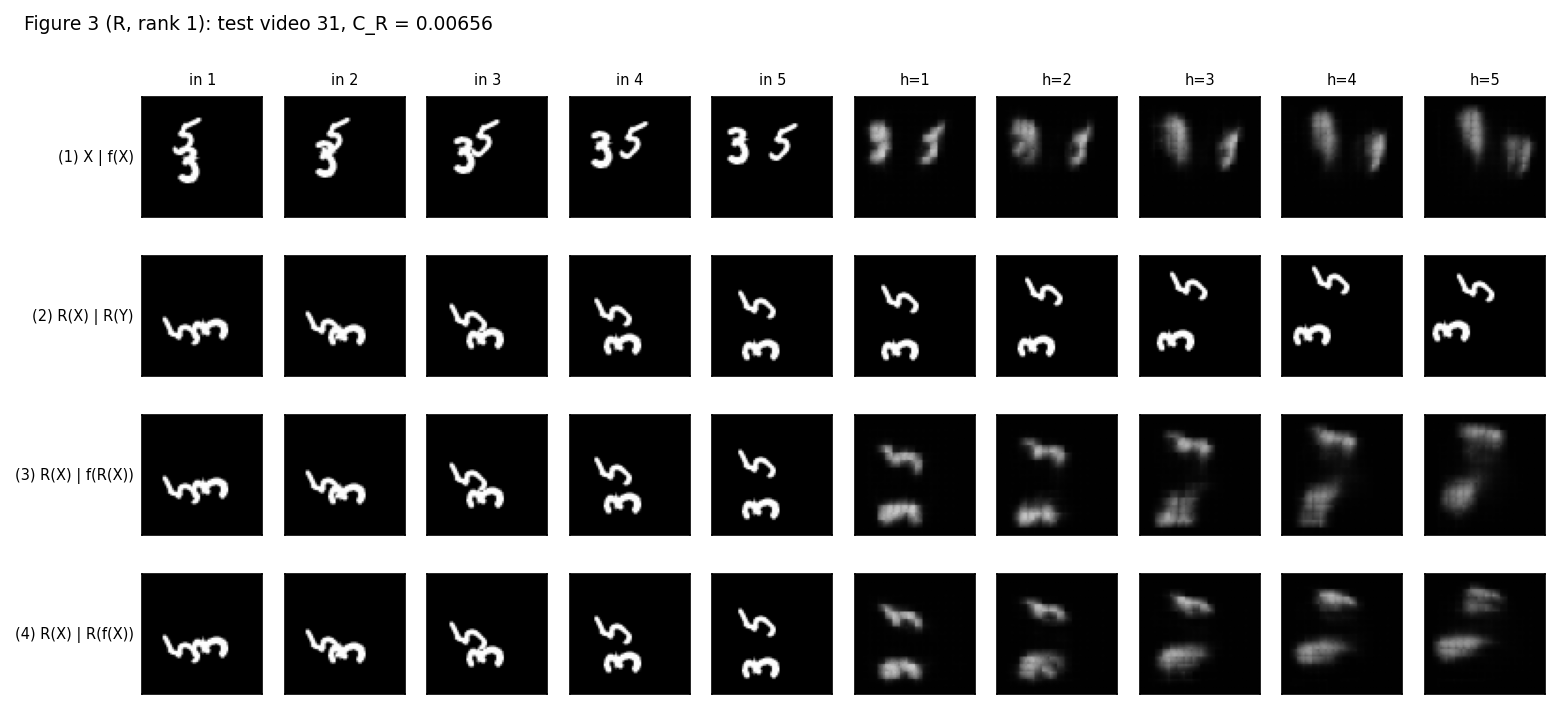
\includegraphics[width=0.93\textwidth]{fig/figure3_R_rank1_video31.png}\\[2pt]
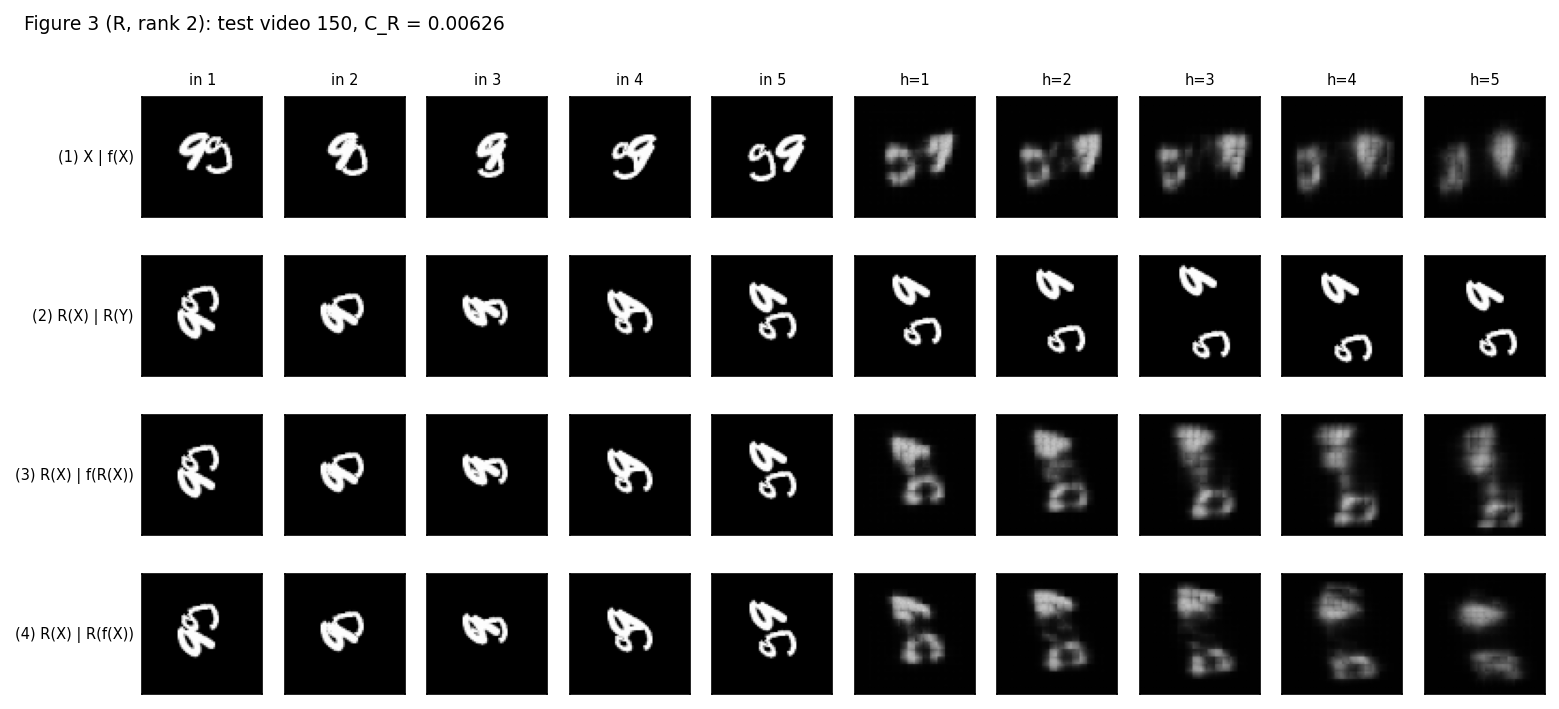
\includegraphics[width=0.93\textwidth]{fig/figure3_R_rank2_video150.png}
\caption*{\textbf{Figure 3 (part 2).} The two test videos with the largest per-video $C_R$ for the seed-0 model A (videos 31 and 150). Rows as in part 1 with $T=R$. GIFs: \texttt{gifs/figure3\_R\_rank1\_video31.gif}, \texttt{gifs/figure3\_R\_rank2\_video150.gif}.}
\end{figure}

\begin{figure}[H]
\centering
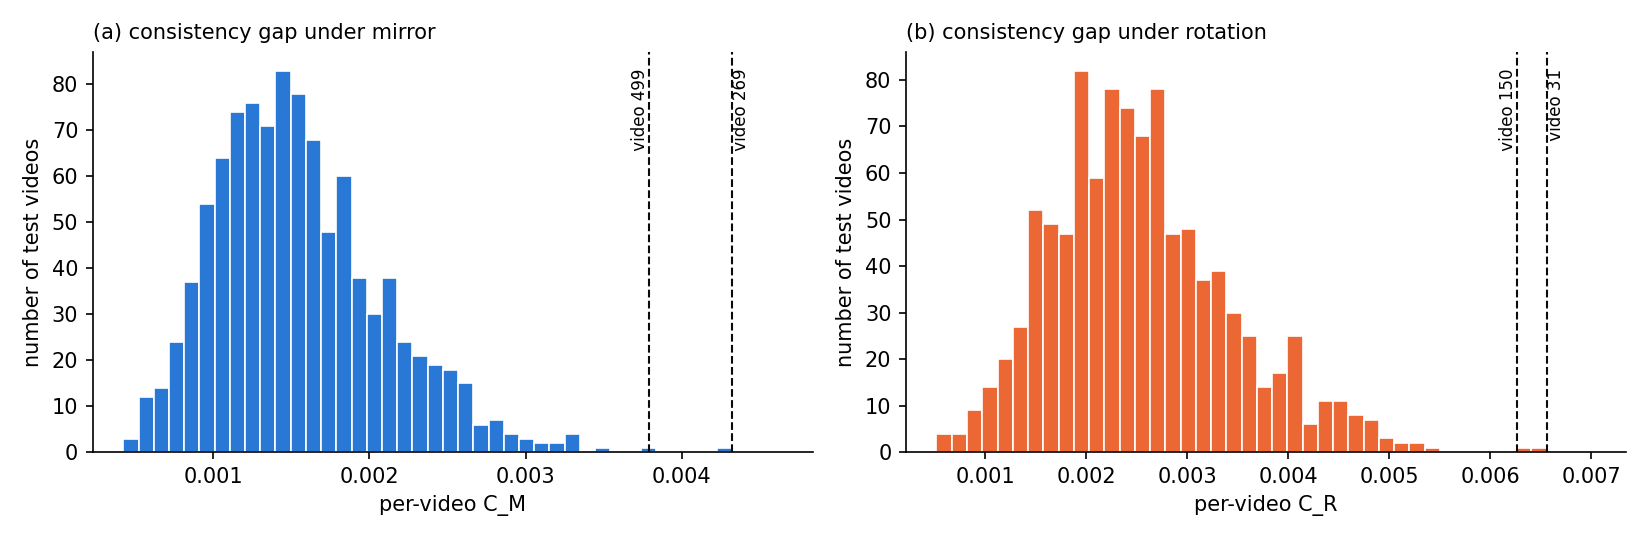
\includegraphics[width=\textwidth]{fig/figure4.png}
\caption*{\textbf{Figure 4.} Histograms of the per-video $C_M$ (a) and $C_R$ (b) of the seed-0 model A over the 1,000 test videos; dashed lines mark the Figure 3 videos.}
\end{figure}

\qa{Q2.6}
Blank and Copy-last have $C_M=C_R=0$ exactly (Table 3), yet they are the two worst predictors: their errors are 0.0426 and 0.0641, compared with 0.0222 for model A. They are consistent for a trivial reason: Blank ignores the input completely (a black frame mirrored or rotated is still a black frame), and Copy-last only repeats the last input frame, and copying a frame gives the same result whether one transforms before or after. Neither of them has learned anything about motion. So $C_T$ on its own only tells us whether a model treats a transformed video in the same way as the original; it does not tell us whether the predictions are correct. Read alone, $C_T$ would even rank Blank ($C_M=0$) above model A ($C_M=0.00163$), which is clearly wrong; in the same way, a model that outputs a uniform grey frame would be perfectly consistent and useless. This is why $E_T$ must always be reported next to $C_T$: $E_T$ compares the prediction on the transformed video with the true transformed future $T(Y)$, so it measures correctness. A good model needs both a small $C_T$ (consistent) and an $E_T$ close to its normal error $E$ (correct). Only the reverse direction comes for free: since $T$ only rearranges pixels, $C_T\le2(E_T+E)$, so a model that is accurate on both the original and the transformed videos must also be fairly consistent, but a consistent model need not be accurate. (Per pixel, with $a=f(T(X))-T(Y)$ and $b=T(Y)-T(f(X))$: $(a+b)^2\le2a^2+2b^2$; $a^2$ averages to $E_T$, and since $T$ only moves pixels, $b^2$ averages to $E$.)

\qa{Q2.7}
In test video 150 under rotation (Figure 3, $R$ rank 2, $C_R=0.00626$), rows 3 and 4 disagree about the upper digit, the rotated 9. In the true future (row 2), this digit stays near the top of the frame and drifts only slightly to the right. When model A predicts on the original video and the prediction is rotated afterwards (row 4), the digit stays near the top as a wide, blurry blob, which agrees with the truth on where the digit is, although its shape is lost. When model A predicts directly on the rotated video (row 3), its account of the motion changes: from $h=3$ on, the digit's brightness spreads downwards into a tall vertical streak that reaches towards the lower digit, so the digit blurs into something unrecognisable and the model behaves as if it might be moving down, which it is not. The lower digit moves to the right in a similar way in rows 3 and 4, so the disagreement comes almost entirely from the upper digit. In the first input frames the two 9s overlap, which may explain why the model is unsure which piece belongs to which digit; the other three videos in Figure 3 also start with overlapping digits.

\qa{Q2.8}
Yes, rotation is harder than mirroring for model A, although both effects are small. Under mirroring the error rises from $E=0.0222$ to $E_M=0.0228$ (+3\%), and under rotation to $E_R=0.0240$ (+8\%), so rotation's extra error (0.0018) is about three times mirroring's (0.0006). The consistency gap is also larger, $C_R=0.00288$ against $C_M=0.00163$, and both seeds show the same ordering, so this is not seed noise. The difference does not come from the motion: in Q2.1 every direction already occurs in training, and both transformations only move directions between familiar bins while keeping the speed the same, so motion under rotation is no less familiar than under mirroring. Using the Figure 1(a) bins, about 13\% of the direction distribution moves to a different bin under the mirror and about 16\% under rotation, a similar change that cannot explain an extra error about three times larger. What differs is the appearance (Q2.2): a mirror keeps vertical strokes vertical, and nearly symmetric digits such as 0, 1 and 8 hardly change, whereas a 90$^\circ$ rotation turns every digit on its side, making it wider than tall, unlike any training digit. Figure 3 supports this: in videos 31 and 150 the true rotated digits are wide, yet when model A runs on the rotated video (row 3) it draws some of them as tall or tilted streaks, the shape of upright digits, while when it runs on the original video and its output is rotated (row 4), the blobs stay wide like the truth. Model A's motion rule therefore seems partly tied to what upright digits look like, which is why the transformation that changes appearance more costs more. In Q2.5 I predicted the same result for both; the results show they are close, but rotation is measurably harder.

\begin{table}[H]
\centering\small
\begin{tabular}{@{}lccccc@{}}
\toprule
\textbf{Model} & \textbf{$E^{(2)}$ 1$\times$} & \textbf{$E^{(2)}$ 2$\times$} & \textbf{$E^{(2)}$ 3$\times$} & \textbf{$E^{(5)}$ 1$\times$} & \textbf{$E^{(5)}$ 2$\times$} \\
\midrule
A & \makecell{0.0189\\[-1pt]{\tiny(0.0191, 0.0186)}} & \makecell{0.0442\\[-1pt]{\tiny(0.0435, 0.0449)}} & \makecell{0.0511\\[-1pt]{\tiny(0.0509, 0.0514)}} & \makecell{0.0222\\[-1pt]{\tiny(0.0225, 0.0220)}} & \makecell{0.0484\\[-1pt]{\tiny(0.0476, 0.0493)}} \\
Copy-last & 0.0548 & 0.0661 & 0.0703 & 0.0641 & 0.0719 \\
\bottomrule
\end{tabular}
\caption*{\textbf{Table 4.} Faster motion ($t=1$). Across speeds only $E^{(2)}$ is compared; at 3$\times$ only two targets exist (frames 16, 19). Model A: mean (seed 0, seed 1).}
\end{table}

\begin{figure}[H]
\centering
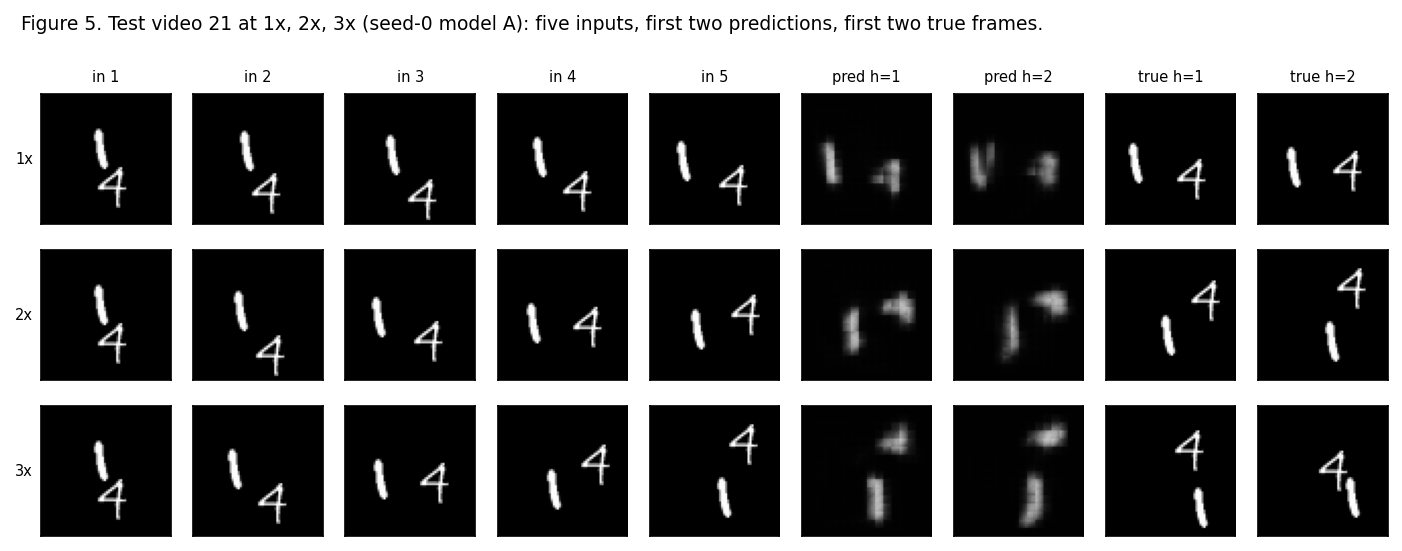
\includegraphics[width=\textwidth]{fig/figure5.png}
\caption*{\textbf{Figure 5.} Test video 21 at 1$\times$, 2$\times$ and 3$\times$ (seed-0 model A): five inputs, first two predictions, first two true frames. The digits do not overlap in the displayed true frames.}
\end{figure}

\qa{Q2.9}
Model A's predictions fall apart already at 2$\times$. $E^{(2)}$ rises from 0.0189 at 1$\times$ to 0.0442 at 2$\times$ (2.3 times higher) and 0.0511 at 3$\times$ (Table 4). Blank's error is about 0.0426 at every horizon (Table 2), so from 2$\times$ on model A is no better than predicting black frames, and its $E^{(5)}$ at 2$\times$ (0.0484) is worse than Blank; it still beats Copy-last (0.0661 at 2$\times$).

This does \emph{not} agree with my reach estimate. At 2$\times$ the digits move 6.64 px per step, inside the 8 px reach, so by reach alone model A should cope at 2$\times$ and only fail at 3$\times$ (9.96 px). The estimate missed two things. First, reach is only an upper limit: the most the architecture \emph{could} move information in one step, not what it actually learned. Model A was trained only at 1$\times$, where digits move about 3.3 px per step, less than one grid cell, so it never needed to move information further than about one cell per step and never learned to use its full reach. Second, the 8 px path uses the outermost weights of the $3\times3$ kernels in both layers; in practice information near the edge of a kernel's window is carried only weakly, so the useful reach is smaller than the theoretical one.

Figure 5 (test video 21) shows what the failure looks like. At 1$\times$ the predicted blobs are blurry but sit where the true digits are. At 2$\times$ and 3$\times$ the predicted digits \emph{stall}: at $h=1$ and $h=2$ they stay close to where they were in the last input frame, while the true digits have moved much further (the 1 moves right; at 3$\times$ the 4 bounces and comes back down, but the predicted 4 stays at the top). They also \emph{blur}: the 1 becomes a long vertical smear and the 4 a shapeless blob. No digit vanishes or is duplicated. Stalling suggests the model does not pick up the large velocity: it cannot link a digit's old and new positions when they are far apart, so it falls back on the slow motion it learned in training, or none at all. Blur suggests it is unsure where the digit is going and spreads it over the possible positions, which costs less under squared error than a sharp wrong guess. A vanishing digit would mean the model had lost track of it completely, and a duplicated digit would mean it treated the old and new positions as two different objects; neither happens here, so the model still knows a digit is there, but not how fast it moves.

\qa{Q2.10}
No. Model A was trained only at 1$\times$ and has a fixed reach of 8 px, so on fast videos both causes are present at once, and both predict a failure; its results alone cannot tell them apart. The failure at 2$\times$, which is inside the reach, hints that unfamiliar motion matters, but it does not prove it, because the useful reach may be smaller than the theoretical 8 px (Q2.9). To separate the two causes, change one thing at a time, as in a controlled experiment. First, train the same architecture on mixed speeds ($k$ drawn uniformly from \{1, 2, 3\}): fast motion is then no longer unfamiliar, while the reach stays at 8 px. If this model works at 2$\times$ and 3$\times$, the failure was caused by unfamiliar motion; if it works at 2$\times$ but still fails at 3$\times$, where digits move 9.96 px per step, beyond the 8 px reach, the remaining failure is architectural. Second, to confirm this, train a network with a larger reach (e.g.\ bigger kernels, dilated convolutions or a bigger patch) on the same mixed speeds: if it fixes 3$\times$ where the same-reach model fails, the cause was reach, because more training data cannot carry information further than the architecture allows.

%=====================================================================
\subsection{What can data fix?}

\qa{Q2.11} \emph{(written before training models B--D; reproduced unedited)}

I predict that model B, trained with random mirrors and rotations, will fix the rotation (and mirror) failure, because it sees transformed digits during training. I predict that model C, trained on mixed speeds, will fix the failure at 2$\times$. I predict that the failure at 3$\times$ will be fixed by both model C and model D.

\textbf{Model D (design).} Identical to model A except that the $3\times3$ convolution of the second ConvLSTM layer is \emph{dilated by 3} (padding 3). Code:
\texttt{self.cell2.conv = nn.Conv2d(128, 256, kernel\_size=3, padding=3, dilation=3)}.

\begin{table}[H]
\centering\small
\begin{tabular}{@{}lccccc@{}}
\toprule
\textbf{Model} & \textbf{from $u_\tau$} & \textbf{from $h^{(1)}_{\tau-1}$} & \textbf{from $h^{(2)}_{\tau-1}$} & \textbf{reach (longest)} & \textbf{Params}\\
\midrule
A & 2 cells = 8 px & 2 cells = 8 px & 1 cell = 4 px & \textbf{8 px} & 480,784\\
D & 4 cells = 16 px & 4 cells = 16 px & 3 cells = 12 px & \textbf{16 px} & 480,784\\
\bottomrule
\end{tabular}
\caption*{\textbf{Table S1.} One-step reach \emph{measured} with a gradient check (one step of the untrained network; every input cell with a non-zero gradient for one output cell). For D, every horizontal and vertical offset from $-4$ to $+4$ cells is reachable (no holes).}
\end{table}

\begin{table}[H]
\centering\small
\begin{adjustbox}{max width=\textwidth}
\begin{tabular}{@{}lccccc@{}}
\toprule
\textbf{Model} & \textbf{$E^{(5)}$ 1$\times$} & \textbf{$C_M$} & \textbf{$E_M$} & \textbf{$C_R$} & \textbf{$E_R$} \\
\midrule
A & \makecell{0.0222\\[-1pt]{\tiny(0.0225, 0.0220)}} & \makecell{0.00163\\[-1pt]{\tiny(0.00155, 0.00171)}} & \makecell{0.0228\\[-1pt]{\tiny(0.0231, 0.0226)}} & \makecell{0.00288\\[-1pt]{\tiny(0.00254, 0.00321)}} & \makecell{0.0240\\[-1pt]{\tiny(0.0240, 0.0239)}} \\
B & \makecell{0.0229\\[-1pt]{\tiny(0.0233, 0.0224)}} & \makecell{0.00111\\[-1pt]{\tiny(0.00106, 0.00115)}} & \makecell{0.0229\\[-1pt]{\tiny(0.0234, 0.0224)}} & \makecell{0.00134\\[-1pt]{\tiny(0.00141, 0.00128)}} & \makecell{0.0228\\[-1pt]{\tiny(0.0232, 0.0223)}} \\
C & \makecell{0.0267\\[-1pt]{\tiny(0.0272, 0.0263)}} & \makecell{0.00135\\[-1pt]{\tiny(0.00117, 0.00154)}} & \makecell{0.0269\\[-1pt]{\tiny(0.0273, 0.0265)}} & \makecell{0.00258\\[-1pt]{\tiny(0.00220, 0.00295)}} & \makecell{0.0279\\[-1pt]{\tiny(0.0282, 0.0276)}} \\
D & \makecell{0.0285\\[-1pt]{\tiny(0.0291, 0.0280)}} & \makecell{$7.74\times10^{-4}$\\[-1pt]{\tiny($7.11\times10^{-4}$, $8.38\times10^{-4}$)}} & \makecell{0.0286\\[-1pt]{\tiny(0.0291, 0.0281)}} & \makecell{0.00171\\[-1pt]{\tiny(0.00142, 0.00199)}} & \makecell{0.0293\\[-1pt]{\tiny(0.0297, 0.0289)}} \\
\bottomrule
\end{tabular}
\end{adjustbox}
\caption*{\textbf{Table 5 (part a).} Models A--D at 1$\times$ (test set, $t=1$): accuracy and consistency. Entries: mean (seed 0, seed 1).}
\end{table}

\begin{table}[H]
\centering\small
\begin{adjustbox}{max width=\textwidth}
\begin{tabular}{@{}lcccccc@{}}
\toprule
\textbf{Model} & \textbf{$E^{(2)}$ 1$\times$} & \textbf{$E^{(2)}$ 2$\times$} & \textbf{$E^{(2)}$ 3$\times$} & \textbf{Parameters} & \textbf{\makecell{Train time\\per epoch (s)}} & \textbf{\makecell{Inference\\time (s)}} \\
\midrule
A & \makecell{0.0189\\[-1pt]{\tiny(0.0191, 0.0186)}} & \makecell{0.0442\\[-1pt]{\tiny(0.0435, 0.0449)}} & \makecell{0.0511\\[-1pt]{\tiny(0.0509, 0.0514)}} & 480,784 & \makecell{11.0\\[-1pt]{\tiny(10.9, 11.2)}} & \makecell{0.386\\[-1pt]{\tiny(0.387, 0.386)}} \\
B & \makecell{0.0192\\[-1pt]{\tiny(0.0197, 0.0187)}} & \makecell{0.0431\\[-1pt]{\tiny(0.0433, 0.0429)}} & \makecell{0.0490\\[-1pt]{\tiny(0.0496, 0.0483)}} & 480,784 & \makecell{10.8\\[-1pt]{\tiny(10.8, 10.9)}} & \makecell{0.388\\[-1pt]{\tiny(0.387, 0.388)}} \\
C & \makecell{0.0232\\[-1pt]{\tiny(0.0237, 0.0227)}} & \makecell{0.0288\\[-1pt]{\tiny(0.0292, 0.0285)}} & \makecell{0.0333\\[-1pt]{\tiny(0.0335, 0.0331)}} & 480,784 & \makecell{10.5\\[-1pt]{\tiny(10.5, 10.5)}} & \makecell{0.389\\[-1pt]{\tiny(0.388, 0.390)}} \\
D & \makecell{0.0259\\[-1pt]{\tiny(0.0264, 0.0254)}} & \makecell{0.0296\\[-1pt]{\tiny(0.0300, 0.0292)}} & \makecell{0.0332\\[-1pt]{\tiny(0.0335, 0.0328)}} & 480,784 & \makecell{14.8\\[-1pt]{\tiny(14.8, 14.8)}} & \makecell{0.549\\[-1pt]{\tiny(0.548, 0.549)}} \\
\bottomrule
\end{tabular}
\end{adjustbox}
\caption*{\textbf{Table 5 (part b).} Models A--D: speed and cost (T4 GPU). Training time per epoch from the training logs; inference time = predicting all 1,000 original test videos at batch size 32 under \texttt{eval()} and \texttt{no\_grad()}, measured in one session for all models.}
\end{table}

\begin{figure}[H]
\centering
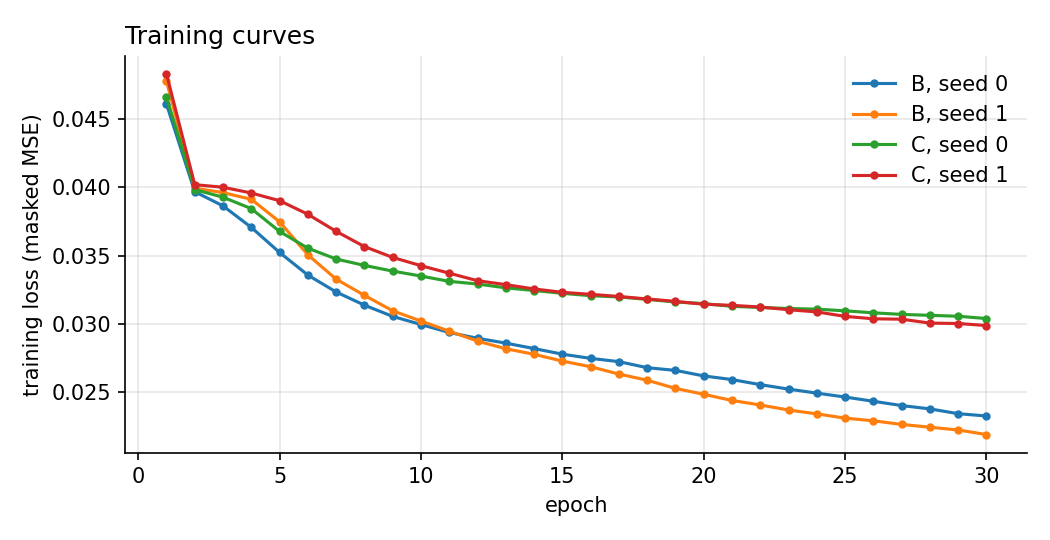
\includegraphics[width=0.49\textwidth]{fig/curves_BC.png}\hfill
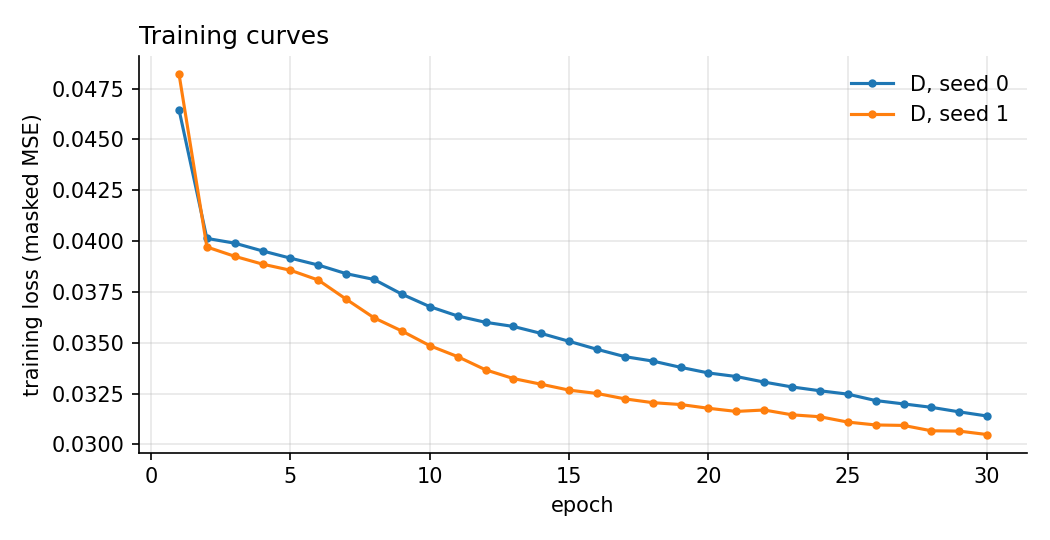
\includegraphics[width=0.49\textwidth]{fig/curves_D.png}
\caption*{\textbf{Figure S2.} Training loss of models B, C (left) and D (right). Models C and D are trained on mixed speeds, so their training loss is higher than B's; D is still improving at epoch 30. (Supplementary.)}
\end{figure}

\qa{Q2.12}
Model D is model A with a single change: the $3\times3$ convolution of the second ConvLSTM layer is dilated by 3, with padding 3 so the grid stays $16\times16$. Everything else is identical: patch size 4 (\texttt{pixel\_unshuffle}/\texttt{pixel\_shuffle}), two ConvLSTM layers with 64 hidden channels, the $1\times1$ output convolution, the 9-step rollout without teacher forcing, and the training protocol (mixed speeds, like model C). A dilated $3\times3$ kernel uses the same 9 weights but places them 3 cells apart, so it costs no extra parameters: D has exactly 480,784 parameters, the same as A and C and well under the 721,176 limit. I chose this design so that D differs from C \emph{only in reach}, not in size: if D beats C, the reason cannot be extra parameters.

Reach, counted as in Q2.3: one grid cell is 4 px, and only the $3\times3$ convolutions move information (the gates, unshuffle/shuffle and the $1\times1$ head move nothing). In layer 1 the ordinary $3\times3$ convolution moves information at most 1 cell; in layer 2 the dilated convolution moves it at most 3 cells. The path from $u_\tau$ therefore moves $1+3=4$ cells, the path from $h^{(1)}_{\tau-1}$ also $1+3=4$ cells, and the path from $h^{(2)}_{\tau-1}$ 3 cells. The longest path is 4 cells $=$ \textbf{16 px} along rows and columns (about 22.6 px diagonally), strictly larger than model A's 8 px and above the 9.96 px per step of 3$\times$ motion. Because layer 1 moves information by $-1,0,+1$ cells and layer 2 by $-3,0,+3$, together they reach every offset from $-4$ to $+4$ cells, so there are no holes (unlike dilation 2 in both layers, which would reach only even offsets). A gradient check (Table S1) confirms this: one step reaches 8 px for model A and 16 px for model D, with every offset from $-4$ to $+4$ cells reachable.

\qa{Q2.13}
Each label is supported by a comparison in Table 5 in which only one thing changes.
\begin{itemize}
\item \textbf{Rotation (and the small mirror gap): appearance.} Model B differs from A only by symmetry augmentation, i.e.\ by showing it mirrored and rotated digits during training. This alone reduces the extra error under rotation from +0.0018 (A: $E_R=0.0240$ vs.\ $E=0.0222$) to about zero (B: $E_R=0.0228$ vs.\ $E=0.0229$); the small mirror gap also disappears (+0.0006 $\to$ 0.0000), and the consistency gaps drop ($C_R$ 0.00288 $\to$ 0.00134, $C_M$ 0.00163 $\to$ 0.00111). The motion was already familiar (Q2.1), so what B added was new digit appearances. B leaves the speed failures unchanged ($E^{(2)}$ at 2$\times$: 0.0431 vs.\ 0.0442), which confirms that the two problems are separate.
\item \textbf{2$\times$: unfamiliar motion.} Model C has the same architecture and the same 8 px reach as A; only its training speeds differ. This alone lowers $E^{(2)}$ at 2$\times$ from 0.0442 to 0.0288 ($-35\%$). The digits move 6.64 px per step, inside the reach, so the network could always connect the positions; it had simply never been trained on this motion.
\item \textbf{3$\times$: mainly unfamiliar motion, not reach.} The comparison A$\to$C again gives the large gain ($E^{(2)}$ at 3$\times$: 0.0511 $\to$ 0.0333, $-35\%$). The comparison C$\to$D changes only the architecture, doubling the reach from 8 to 16 px with the same parameters and data, and gives no further gain (0.0333 vs.\ 0.0332). So in these results reach was not what limited the model at 3$\times$, even though 9.96 px per step is above 8 px along an axis. Possible reasons (my interpretation): digit strokes are wide, so a digit's old and new positions still partly overlap within 8 px; the diagonal reach is up to about 11.3 px; and constant velocity can be estimated across several steps. Two caveats: C's error at 3$\times$ is still clearly higher than at 1$\times$ (0.0333 vs.\ 0.0232), so 3$\times$ is improved, not solved; and D's training curve was still falling at epoch 30 (Figure S2), so a longer-trained D might show some benefit.
\end{itemize}
If model C had still done badly at 3$\times$ while model D did well, that would have shown that the 3$\times$ failure was architectural reach: C had seen 3$\times$ motion in training and still failed, and only the larger reach fixed it. More training data cannot get past that limit, because training only changes the numbers inside each kernel, while the set of cells that can affect an output in one step is fixed by the kernel size, dilation, patch size and number of layers. If a digit moves further than that in one step, there is no path in the network connecting its old position (in the state) with its new position; the gradient of the output with respect to those far-away inputs is exactly zero, so no amount of data can teach the network to use them.

\qa{Q2.14}
Yes. Every change cost some accuracy on the original 1$\times$ clips ($E^{(5)}$ at 1$\times$, Table 5): B slightly (0.0229 vs.\ 0.0222, +3\%), C clearly (0.0267, +20\%) and D the most (0.0285, +28\%).
\begin{itemize}
\item \textbf{B: worth it.} For +3\% at 1$\times$ it removes the rotation gap ($E_R-E$ from +0.0018 to $-0.0001$) and halves $C_R$.
\item \textbf{C: worth it whenever the model has to handle faster motion}, which is the point of this assignment; it would not be worth it for a forecaster that only ever sees normal-speed videos. The cost at 1$\times$ (+0.0045 in $E^{(5)}$) buys much larger gains at 2$\times$ ($E^{(2)}$ $-0.0154$) and 3$\times$ ($-0.0178$); at those speeds A was no better than predicting black frames, while C is well below that level. The 1$\times$ cost is expected (interpretation): only a third of C's training windows are at 1$\times$, and the same weights must now cover three speeds, so the model hedges more.
\item \textbf{D: not worth it here.} Compared with C, which has the same training data, it is worse at 1$\times$ (0.0285 vs.\ 0.0267), no better at 2$\times$ (0.0296 vs.\ 0.0288) or 3$\times$ (0.0332 vs.\ 0.0333), and about 40\% slower to train (14.8 vs.\ 10.5 s per epoch) and to run (0.549 vs.\ 0.389 s). A likely reason for its 1$\times$ loss (interpretation): layer 2's dilated kernel only links cells that are 0 or 3 apart, so small 1$\times$ movements (less than one cell per step) can be handled only by layer 1, and D's predictions look blockier (Figure 6); D was also still improving at epoch 30.
\end{itemize}

%=====================================================================
\subsection{The final model}

\textbf{Why the symmetrised forecaster is exactly consistent.} Take any trained $f$ and any $h\in G$. Then $\bar f(h(X))=\frac18\sum_{g\in G}g^{-1}f(ghX)$. Substitute $g'=gh$. Because $G$ is a group, $g\mapsto gh$ maps $G$ one-to-one onto itself, so $g'$ runs over all eight elements exactly once, and $g^{-1}=hg'^{-1}$. Since $h$ only rearranges pixels, it is linear and can be taken out of the average:
\[
\bar f(h(X))=\tfrac18\sum_{g'\in G}h\,g'^{-1}f(g'X)=h\big(\bar f(X)\big).
\]
With $h=M$ and $h=R$ this gives $\bar f(T(X))=T(\bar f(X))$, so $C_M=C_R=0$ exactly for any $f$. (With a subset of $G$ that is not closed, the re-indexed sum would run over different elements and the equality would fail.) In floating point the eight terms are added in a different order, so the measured values are about $10^{-17}$ (Table 6).

\textbf{Choice of final model.} I use the handout's default: model D wrapped as a symmetrised forecaster. I did not train D+B: symmetrisation already makes the model exactly consistent, and Table 5 shows no benefit of D's extra reach that would justify further training of D variants.

\begin{table}[H]
\centering\small
\begin{adjustbox}{max width=\textwidth}
\begin{tabular}{@{}lccccc@{}}
\toprule
\textbf{Model} & \textbf{$E^{(5)}$ 1$\times$} & \textbf{$C_M$} & \textbf{$E_M$} & \textbf{$C_R$} & \textbf{$E_R$} \\
\midrule
symmetrised B & \makecell{0.0223\\[-1pt]{\tiny(0.0227, 0.0218)}} & \makecell{$7.63\times10^{-17}$\\[-1pt]{\tiny($8.24\times10^{-17}$, $7.03\times10^{-17}$)}} & \makecell{0.0223\\[-1pt]{\tiny(0.0227, 0.0218)}} & \makecell{$6.17\times10^{-17}$\\[-1pt]{\tiny($6.68\times10^{-17}$, $5.67\times10^{-17}$)}} & \makecell{0.0223\\[-1pt]{\tiny(0.0227, 0.0218)}} \\
\makecell[l]{symmetrised D\\(final model)} & \makecell{0.0284\\[-1pt]{\tiny(0.0289, 0.0278)}} & \makecell{$6.54\times10^{-17}$\\[-1pt]{\tiny($6.53\times10^{-17}$, $6.55\times10^{-17}$)}} & \makecell{0.0284\\[-1pt]{\tiny(0.0289, 0.0278)}} & \makecell{$5.15\times10^{-17}$\\[-1pt]{\tiny($5.09\times10^{-17}$, $5.21\times10^{-17}$)}} & \makecell{0.0284\\[-1pt]{\tiny(0.0289, 0.0278)}} \\
\bottomrule
\end{tabular}
\end{adjustbox}
\caption*{\textbf{Table 6 (part a).} Symmetrised models at 1$\times$ (test set, $t=1$). $C_M$, $C_R$ in scientific notation. Entries: mean (seed 0, seed 1).}
\end{table}

\begin{table}[H]
\centering\small
\begin{adjustbox}{max width=\textwidth}
\begin{tabular}{@{}lcccccc@{}}
\toprule
\textbf{Model} & \textbf{$E^{(2)}$ 1$\times$} & \textbf{$E^{(2)}$ 2$\times$} & \textbf{$E^{(2)}$ 3$\times$} & \textbf{Parameters} & \textbf{\makecell{Train time\\per epoch (s)}} & \textbf{\makecell{Inference\\time (s)}} \\
\midrule
symmetrised B & \makecell{0.0187\\[-1pt]{\tiny(0.0192, 0.0183)}} & \makecell{0.0425\\[-1pt]{\tiny(0.0427, 0.0423)}} & \makecell{0.0482\\[-1pt]{\tiny(0.0488, 0.0476)}} & 480,784 & \makecell{10.8\\[-1pt]{\tiny(10.8, 10.9)}} & \makecell{3.24\\[-1pt]{\tiny(3.22, 3.26)}} \\
\makecell[l]{symmetrised D\\(final model)} & \makecell{0.0258\\[-1pt]{\tiny(0.0263, 0.0253)}} & \makecell{0.0296\\[-1pt]{\tiny(0.0300, 0.0291)}} & \makecell{0.0331\\[-1pt]{\tiny(0.0335, 0.0327)}} & 480,784 & \makecell{14.8\\[-1pt]{\tiny(14.8, 14.8)}} & \makecell{4.73\\[-1pt]{\tiny(4.69, 4.78)}} \\
\bottomrule
\end{tabular}
\end{adjustbox}
\caption*{\textbf{Table 6 (part b).} Symmetrised models: speed and cost (T4 GPU). Training time is that of the underlying learned model (symmetrisation needs no training); inference time includes all eight transformations, forward passes, inverse transformations and the averaging.}
\end{table}

\begin{figure}[p]
\centering
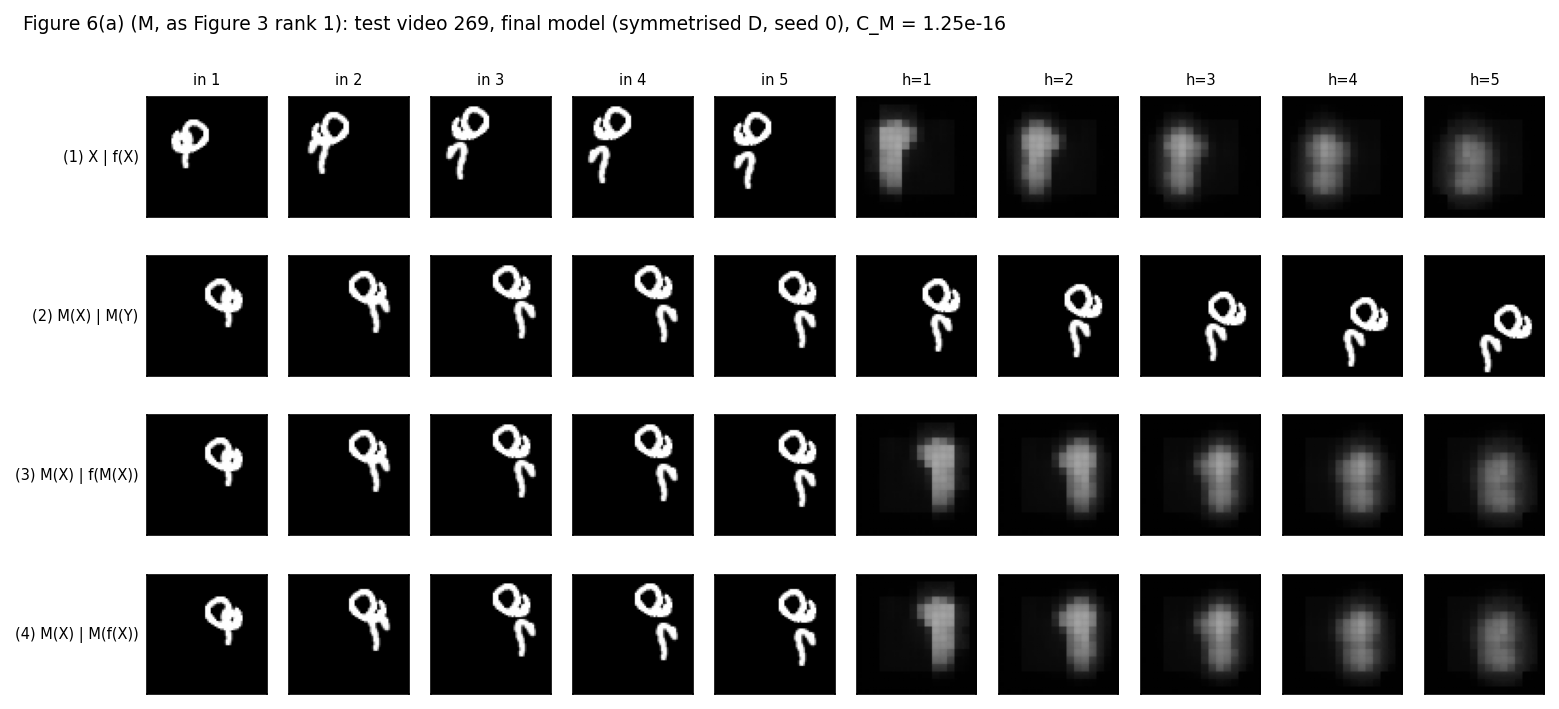
\includegraphics[width=0.93\textwidth]{fig/figure6a_M_rank1_video269.png}\\[2pt]
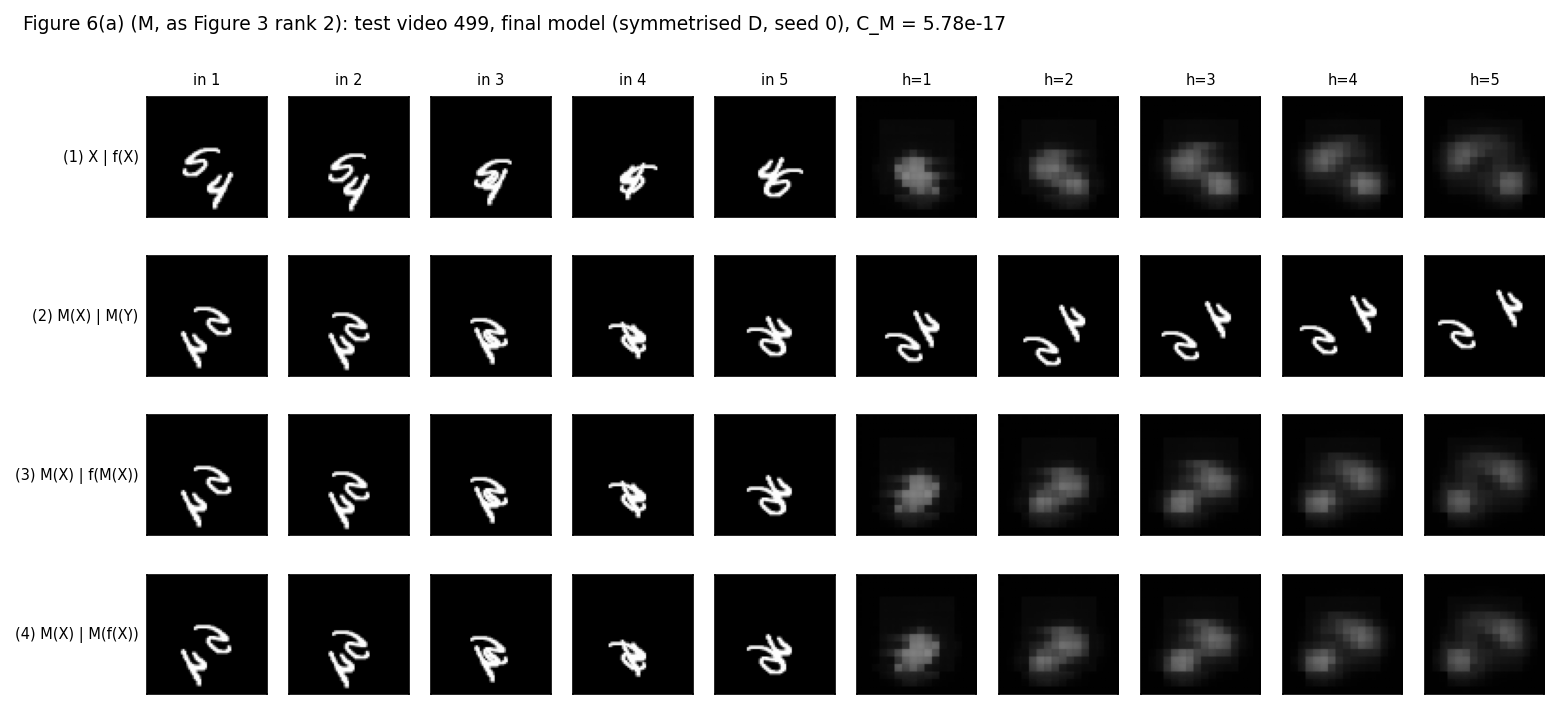
\includegraphics[width=0.93\textwidth]{fig/figure6a_M_rank2_video499.png}
\caption*{\textbf{Figure 6(a), part 1.} Figure 3 repeated with the final model (symmetrised D, seed 0) on the same videos 269 and 499 ($T=M$); rows as in Figure 3. GIFs: \texttt{gifs/figure6a\_M\_rank1\_video269.gif}, \texttt{gifs/figure6a\_M\_rank2\_video499.gif}.}
\end{figure}
\begin{figure}[p]
\centering
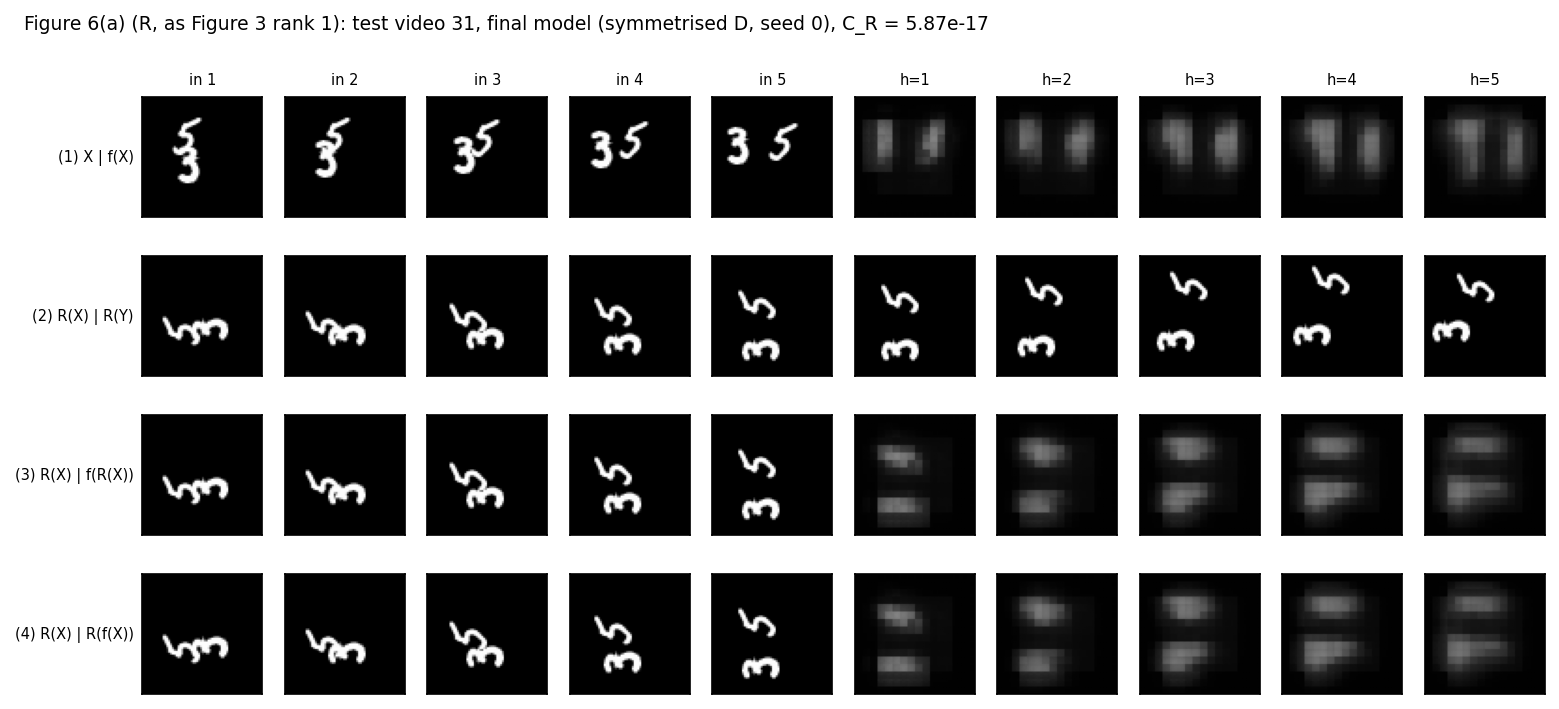
\includegraphics[width=0.93\textwidth]{fig/figure6a_R_rank1_video31.png}\\[2pt]
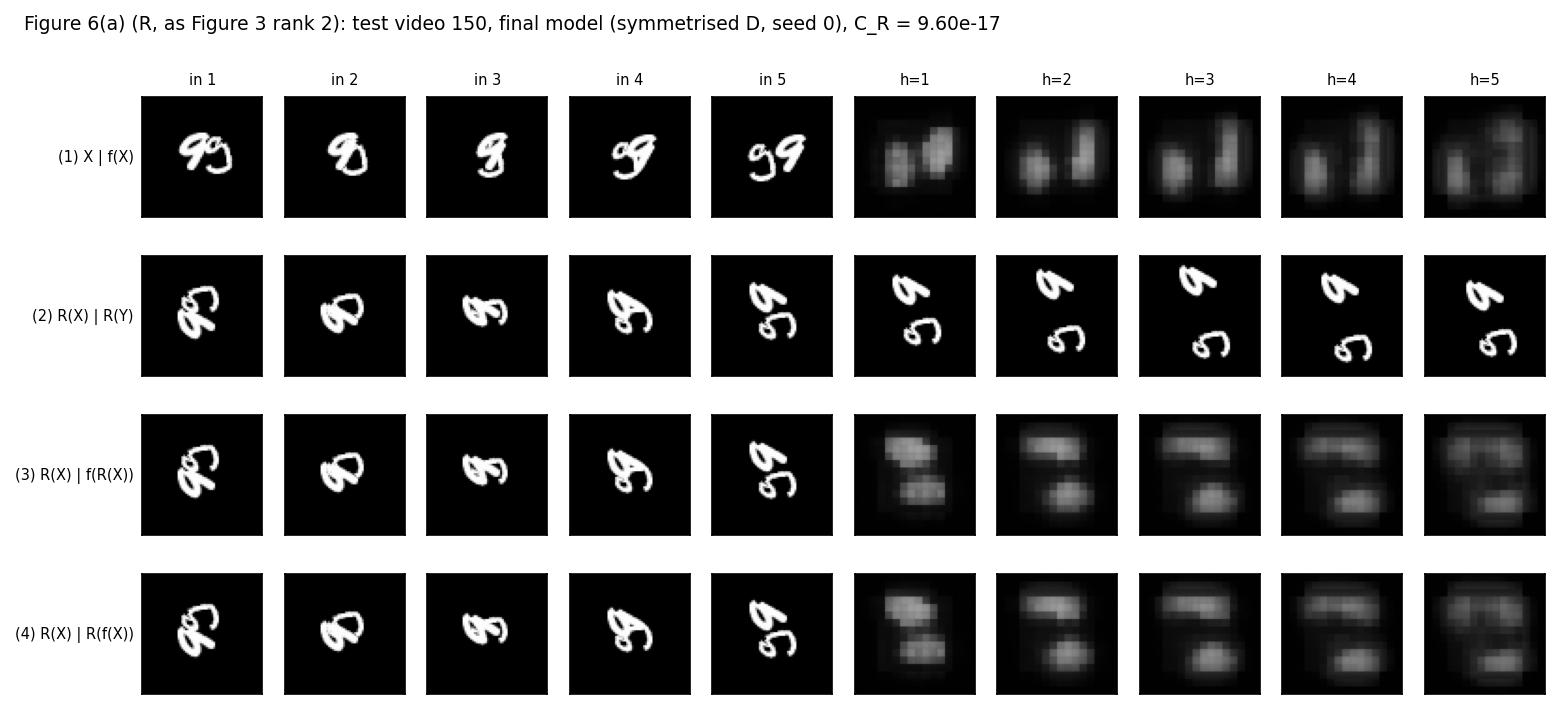
\includegraphics[width=0.93\textwidth]{fig/figure6a_R_rank2_video150.png}
\caption*{\textbf{Figure 6(a), part 2.} Videos 31 and 150 ($T=R$) with the final model. GIFs: \texttt{gifs/figure6a\_R\_rank1\_video31.gif}, \texttt{gifs/figure6a\_R\_rank2\_video150.gif}.}
\end{figure}

\begin{figure}[H]
\centering
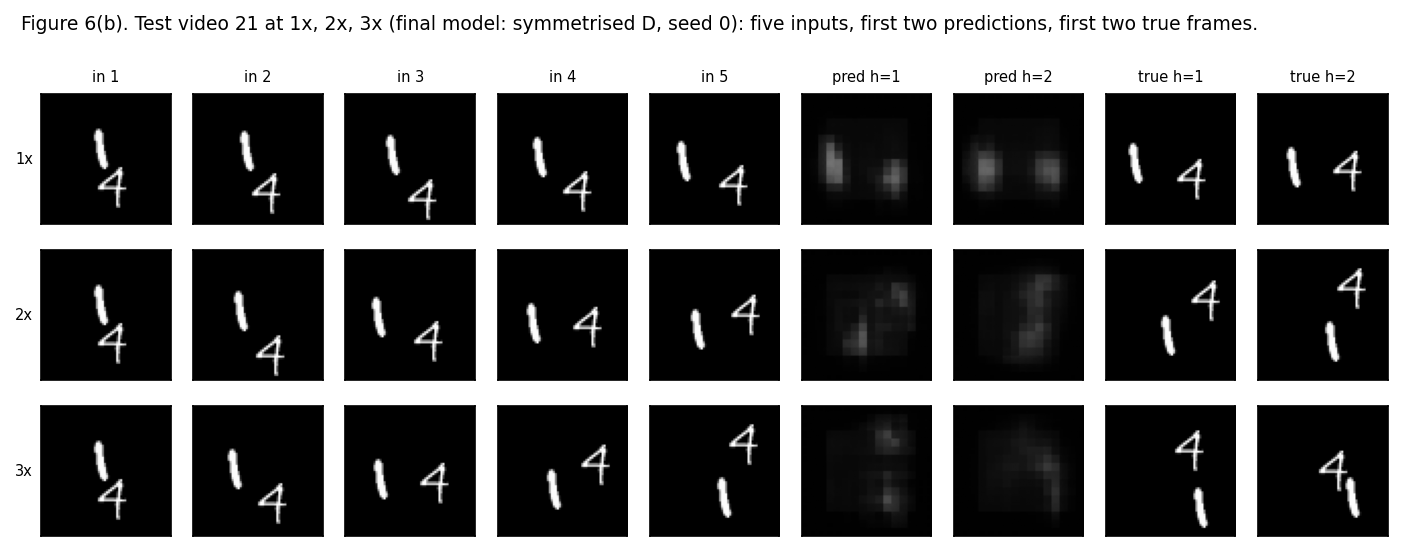
\includegraphics[width=\textwidth]{fig/figure6b.png}
\caption*{\textbf{Figure 6(b).} Figure 5 repeated with the final model (symmetrised D, seed 0) on test video 21.}
\end{figure}

\begin{figure}[H]
\centering
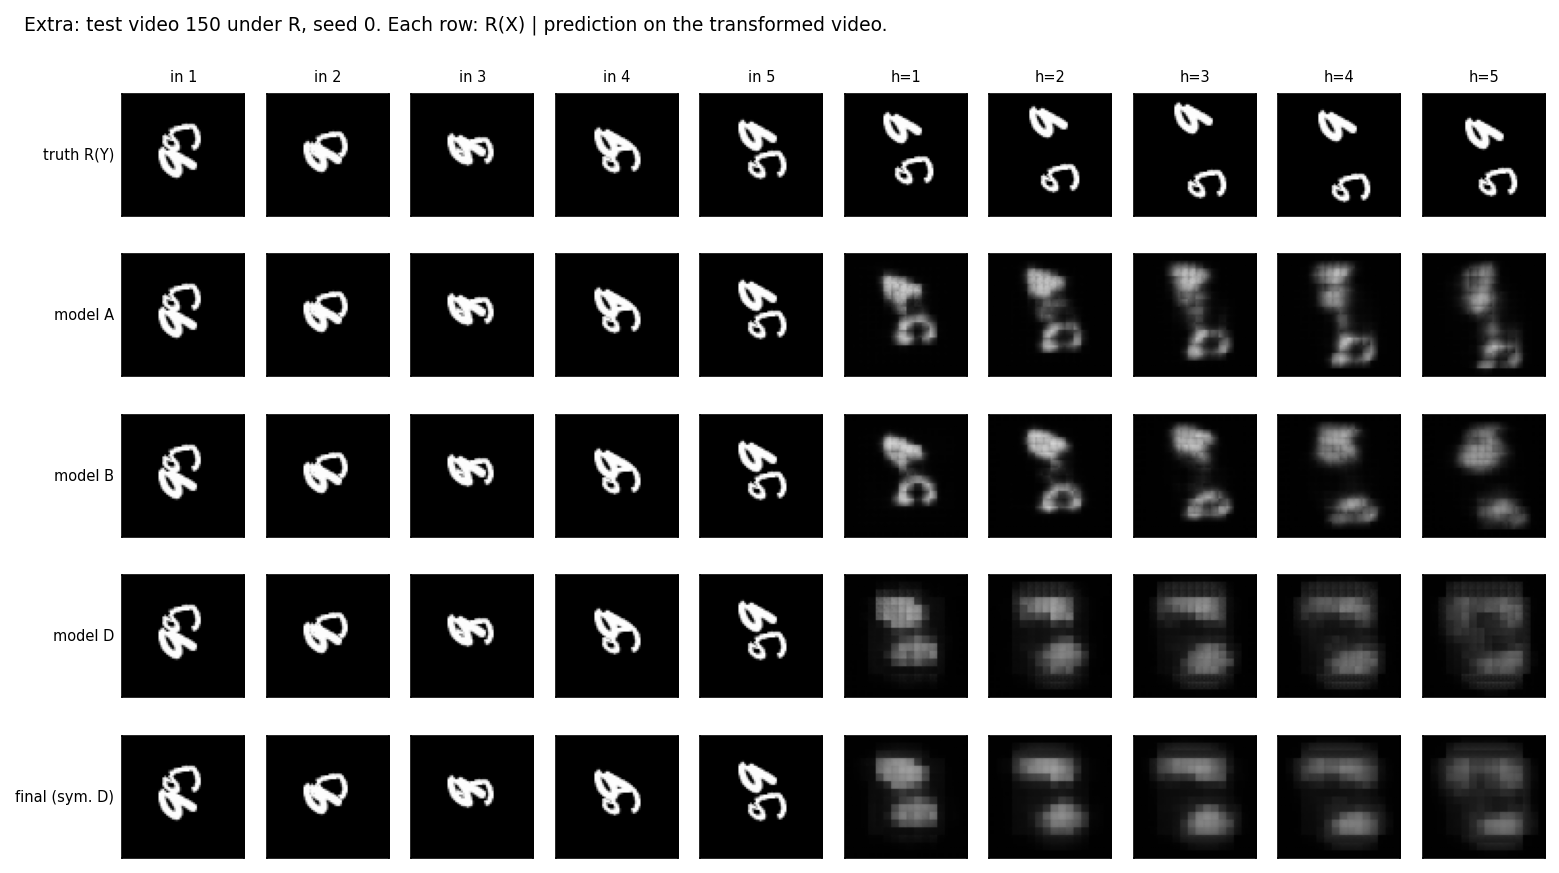
\includegraphics[width=0.95\textwidth]{fig/extra_q27_video150.png}
\caption*{\textbf{Figure S3.} Test video 150 under rotation (seed 0): truth, then the prediction on the rotated video by models A, B, D and the final model. (Supplementary, for Q2.16.)}
\end{figure}

\qa{Q2.15}
\textbf{Consistency.} Learned symmetry (model B) reduces the gaps but does not remove them: from A to B, $C_M$ goes from 0.00163 to 0.00111 and $C_R$ from 0.00288 to 0.00134. Built-in symmetry removes them: symmetrised B and symmetrised D have $C_M$ and $C_R$ of about $10^{-17}$, zero up to floating-point error. Built-in symmetry is exact because of the group argument above, which holds for any $f$ whatever its weights. Learned symmetry is only encouraged: augmentation adds transformed examples to the loss, but with finite training, finite capacity and an optimiser that only lowers the average loss, nothing forces $f(T(X))$ and $T(f(X))$ to be identical for every input.

\textbf{Accuracy.} Because the symmetrised models are exactly equivariant and mirror/rotation only rearrange pixels, their errors on transformed clips equal their errors on original clips exactly: $E_M=E_R=E=0.0223$ for symmetrised B and 0.0284 for symmetrised D. Model B gets close but not exact ($E$ 0.0229, $E_M$ 0.0229, $E_R$ 0.0228). On original clips the symmetrised models are as good as or slightly better than the learned ones: symmetrised B 0.0223 against B's 0.0229 (equal to A's 0.0222, while being far better than A on rotated clips, where A's $E_R$ was 0.0240); symmetrised D 0.0284 against D's 0.0285.

\textbf{Inference cost.} Symmetrisation needs no training but runs the model eight times per prediction: 3.24 s against 0.388 s for B (8.4$\times$) and 4.73 s against 0.549 s for D (8.6$\times$). Symmetry augmentation costs nothing at inference and nothing extra in training (B 10.8 s per epoch vs.\ A 11.0 s).

\textbf{Blur.} Averaging blurs the prediction when the eight predictions disagree. I would expect this when the base model works well only for one orientation (like model A with upright digits), so that seven of the eight predictions are worse and place the digits in slightly different places, or when the data are not truly symmetric (e.g.\ gravity, or digits whose orientation matters), so that forcing symmetry removes useful information. Here it did not hurt: the motion rule and the square box are symmetric under all eight transformations, model B was trained on all eight so its eight predictions already agree closely, and averaging acted like a small eight-member ensemble: $E^{(5)}$ at 1$\times$ went down for B (0.0229 $\to$ 0.0223) and stayed the same for D (0.0285 $\to$ 0.0284). The final model's predictions in Figure 6 are blurry, but mostly because model D's own predictions are blurry and blocky (Figure S3), not because of the averaging.

\qa{Q2.16}
Only partly. In Q2.7, model A's prediction on the rotated video 150 disagreed with its rotated normal prediction (per-video $C_R=0.00626$): the upper digit smeared downward into a tall streak, as if moving towards the lower digit. With the final model (symmetrised D), rows 3 and 4 of Figure 6(a) are identical (per-video $C_R\approx10^{-16}$), and the downward streak is gone: both digits stay as blobs in roughly the right places, the upper one near the top and the lower one drifting right. So the model's account of the motion is now consistent and no longer goes the wrong way. But the prediction is not more accurate: the error on this rotated video is 0.0419 for the final model against 0.0298 for model A, because model D's predictions on this video are much blurrier and blockier, and the digits' shapes are lost. Figure S3 shows which change fixed which part:
\begin{itemize}
\item The wrong-way smear came from appearance: symmetry augmentation (B) already removes most of it, keeping the upper digit near the top and lowering both the error (0.0274) and the consistency gap ($C_R=0.00211$).
\item The remaining disagreement between rows 3 and 4 is removed exactly by symmetrisation, which forces $C_R$ to zero for any model; symmetrised B gives the most accurate version of this video (0.0262).
\item The speed changes did not help here and in fact made this slow (1$\times$) video worse (C 0.0393, D 0.0429): this is the 1$\times$ cost found in Q2.14, larger here because this video, which starts with the two 9s overlapping, is one of the hardest for D (35th worst of 1,000).
\end{itemize}

\qa{Q2.17}
Partly. The final model learned a motion rule that works in every orientation and at all three trained speeds, but only coarsely: digits become blurry blobs. Three pieces of evidence would convince a skeptic. First, controlled comparisons: each change fixed one failure. Symmetry augmentation (B) removed the rotation gap, mixed-speed training (C) cut the 2$\times$ and 3$\times$ errors by about 35\%, and doubling the reach (D) added nothing. Second, exact consistency with low error: $C_M=C_R\approx10^{-17}$ and $E_M=E_R=E=0.0284$, well below Blank (0.0426); consistency alone would not be enough, as Blank shows. Third, at normal speed (Figure 6) the predicted blobs follow the true paths instead of stalling. One test it has not passed: speeds outside training. It was only tested at 1$\times$--3$\times$; a 4$\times$ test needs longer or newly generated videos, so we cannot claim it learned speed in general.
